\documentclass[11pt]{article}

\usepackage[margin=0.85in]{geometry}
\usepackage{amsmath,amssymb}
\usepackage{booktabs}
\usepackage{graphicx}
\usepackage{xcolor}
\usepackage{microtype}
\usepackage[hidelinks]{hyperref}

\definecolor{channelpurple}{HTML}{440154}
\definecolor{channelblue}{HTML}{3B528B}
\definecolor{channelteal}{HTML}{21918C}
\definecolor{channelgreen}{HTML}{5EC962}
\definecolor{channelyellow}{HTML}{FDE725}

\title{What the Colors Mean in the Pythagorean Radial-Gap Plot}
\author{}
\date{}

\begin{document}
\maketitle
\vspace{-2.2em}

The color represents an exact arithmetic label attached to each primitive
Pythagorean triangle.  It does \emph{not} represent the triangle's size or a
dynamical property of the three-body trajectory.

\begin{figure}[h]
  \centering
  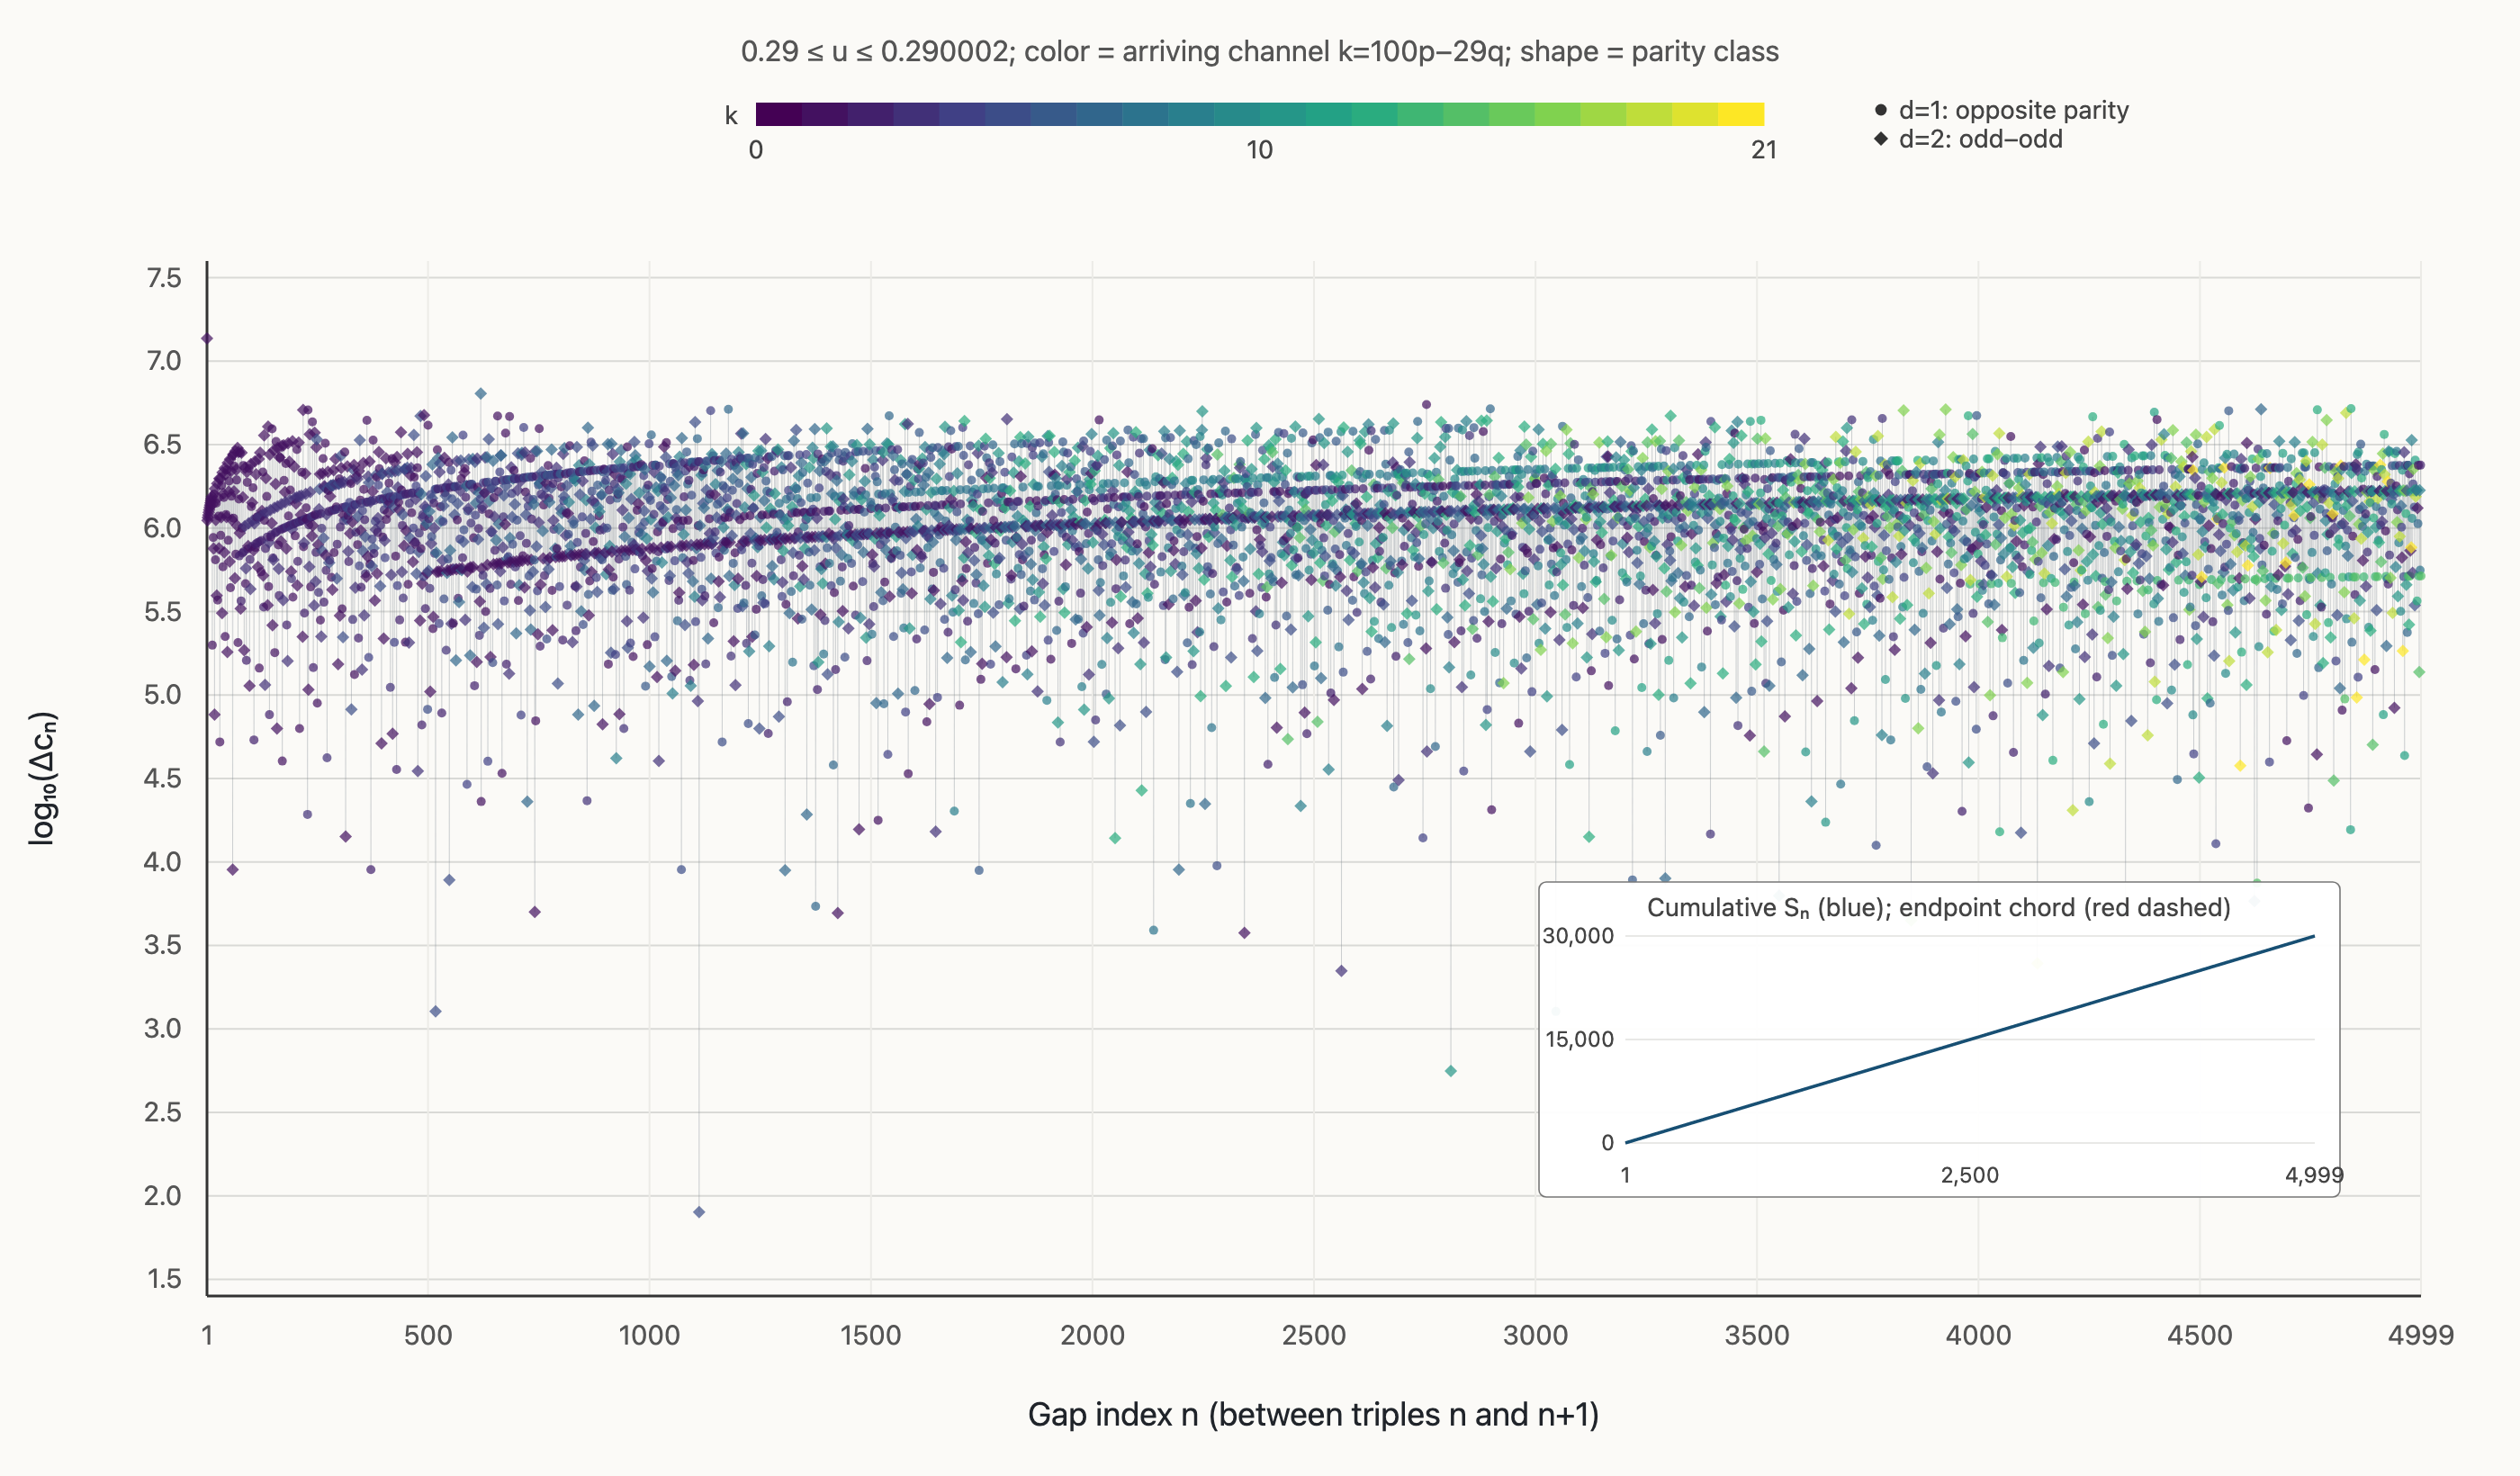
\includegraphics[width=\textwidth]{../plots/log10_primitive_c_gaps_first_5000_colored_channels.png}
  \caption{Successive radial gaps.  Each point is colored using the arriving
  triangle's arithmetic channel.}
\end{figure}

\section*{1. From an actual triangle to its color}

Let
\[
  (x,y,c), \qquad x<y, \qquad x^2+y^2=c^2,
\]
be one of the primitive triples in the narrow wedge.  Its Euclid parameter can
be recovered directly from the three side lengths:
\[
  u=\frac{x}{c+y}.
\]
Reduce this rational number to lowest terms, writing
\[
  u=\frac{p}{q}, \qquad \gcd(p,q)=1.
\]
The color is determined by the integer
\[
  \boxed{k=100p-29q.}
\]

At horizontal index $n$, the plotted height is
\[
  \log_{10}\!\left(c_{n+1}-c_n\right),
\]
and its color is the value of $k$ belonging to the \emph{arriving} triangle
$(x_{n+1},y_{n+1},c_{n+1})$.

\section*{2. Geometric meaning of the channel number}

The lower edge of the parameter interval is $u=29/100$.  Therefore
\[
  \frac{p}{q}-\frac{29}{100}
  =\frac{100p-29q}{100q}
  =\frac{k}{100q}.
\]
Thus $k$ labels parallel rows of rational lattice points immediately above the
lower boundary of the wedge.  Equivalently, it is the integer determinant
\[
  k=\det\!\begin{pmatrix}100&q\\[2pt]29&p\end{pmatrix}.
\]

The color scale in this particular 5,000-triple plot is approximately
\begin{center}
\begin{tabular}{cl}
\toprule
Color & Channel number \\
\midrule
\textcolor{channelpurple}{\rule{1.5em}{0.8em}} Purple & $k\simeq 0$ \\
\textcolor{channelblue}{\rule{1.5em}{0.8em}} Blue & small $k$ \\
\textcolor{channelteal}{\rule{1.5em}{0.8em}} Teal & $k\simeq 10$ \\
\textcolor{channelgreen}{\rule{1.5em}{0.8em}} Green & $k\simeq 15$ \\
\textcolor{channelyellow}{\rule{1.5em}{0.8em}} Yellow & $k\simeq 21$ \\
\bottomrule
\end{tabular}
\end{center}

For example, the first triangle is
\[
  (5800,9159,10841).
\]
It has
\[
  u=\frac{5800}{10841+9159}=\frac{29}{100},
\]
and hence $k=0$.  It lies exactly on the lower endpoint of the wedge and is
colored purple.

\section*{3. Why blue is gradually joined by green}

The upper edge of the interval is
\[
  u\leq \frac{29}{100}+\frac{1}{500000}.
\]
Using $u-29/100=k/(100q)$, this becomes
\[
  \boxed{k\leq\frac{q}{5000}.}
\]
Small triangles have small Euclid denominators $q$, so only small channel
numbers are possible.  For example,
\[
\begin{array}{c|c}
q & \text{largest possible }k \\
\hline
5{,}000 & 1 \\
50{,}000 & 10 \\
100{,}000 & 20
\end{array}
\]

The hypotenuse is approximately proportional to $q^2$.  Moving to the right in
the plot therefore moves toward larger $q$, progressively allowing higher
channel numbers.  Purple and blue dominate at first; teal and green enter as
new channels become arithmetically possible.  The low-$k$ channels have not
vanished---they are increasingly interlaced with the newly available channels.

\section*{4. Meaning of the marker shape}

For reduced $u=p/q$, the primitive triple is
\[
  (x,y,c)=\frac{1}{d}\left(2pq,\;q^2-p^2,\;q^2+p^2\right),
\]
up to ordering the two legs, where
\[
  d=\begin{cases}
      1, & p,q\text{ have opposite parity},\\
      2, & p,q\text{ are both odd}.
    \end{cases}
\]
Consequently, circles in the plot denote $d=1$, while diamonds denote $d=2$.

\section*{5. Channel color versus physical position in the wedge}

The channel number $k$ is not by itself the fractional position across the
physical wedge.  That normalized position is
\[
  \boxed{
  \xi=\frac{u-0.29}{0.000002}=\frac{5000k}{q},
  \qquad 0\leq\xi\leq1.
  }
\]
Thus two triangles with the same $k$ but different $q$ occupy different
fractional positions within the wedge.  The present plot uses $k$ because it
reveals the exact arithmetic strands.  A plot colored by $\xi$ would instead
display each triangle's actual position between the two wedge boundaries.

\end{document}
